\documentclass{tmr}

\usepackage{mflogo}

%include lhs2TeX.fmt
%include lhs2TeX.sty
%include polycode.fmt

\newcommand{\ToDo}[1]{\textbf{ToDo}{#1}}

\title{High Performance Haskell with MPI}
\author{Bernie Pope\email{bjpope@unimelb.edu.au}}
\author{Dmitry Astapov\email{dastapov@gmail.com}}

\newcommand{\Todo}[1]{{\textbf{Todo: #1}}}

\begin{document}

\begin{introduction} 
What is MPI, what is haskell-mpi, how can you use it for writing multi-node programs in Haskell or interoperate with other languages
\end{introduction}

\section{Distributed-memory parallelism}

The World's largest supercomputers now feature hundreds of thousands of CPU cores, and mega-core machines
are just around the corner.\footnote{Mention the LLNL machine in production.} There are many technical
challenges to building such behemoths, but a central problem is
the CPU-to-memory bottleneck. Shared memory parallel computers --- which now dominate consumer-grade
systems --- provide the convenience of one operating system for the whole machine. Even on small
systems the underlying connections between processors and memory are typically non-uniform. Happily for
programmers, shared-memory computers abstract over this inconvenient truth, providing the software
illusion that each core has equivalent access to all the memory banks.
Sadly, it is difficult to scale this abstraction in a
cost-effective way to the supercomputing level; a quick glance at the Top 500 list of supercomputers reveals
no significant large-scale shared-memory systems.\footnote{\url{www.top500.org}}
Instead we see that practically all the listed supercomputers are based on
disributed-memory parallelism; many independent computers (called nodes),
each with their own processors, memory and operating system, connected by one or more high-speed networks.
The nodes themselves are often small multi-core shared-memory computers, so in reality, most supercomputers
are hybrids; nevertheless, the macro architecture is distributed.

Distributed-memory parallelism does not really solve the CPU-to-memory bottleneck (over the whole machine),
afterall sharing data between nodes over a network is a costly operation. Instead it forces programmers to
address the non-uniformity head on, which typically means adopting an explicitly distributed style of
parallel programming.\footnote{There have been several attempts to provide a shared-memory like abstraction
on top of distributed parallel machines, such as Unified Parallel C, but automated load balancing remains
an open problem.} 

\section{Very short intro to MPI and haskell-mpi and outlining the motivation}
What is MPI? If you ever tried to make processes running on separate
computers talk to each other, chances are that you already came across
the MPI or invented parts of it. 

Even though MPI has been standartized only aroung 1995\footnote{Full
  formal definition of protocol, its semantics and reference
  implementation could be found in \cite{mpi-report}}, it has become
de-facto standart in programming on architecures with distributed
memory (``clusters'' or ``parallel computers''). It tries to prove a
language-independent communications means that would allow users to
pass around ``messages'' (hence the name, ``Message Passing
Interface''). We have it on a good authority that MPI is still widely
used today, even though there are numerous alternatives for
inter-process communication. This article would focus on haskell-mpi,
not trying to provide any sort of comparison with possible
alternatives, as authors believe that any choice like this should
ultimately be made in context of the specific task at hand.

So what is, then, haskell-mpi? It is a package of low- and high-level bindings
to C MPI library that allows Haskell programmers to call upon the
powers of MPI with ease. 

What would be the most (stereo)typical use case for haskell-mpi?
Suppose that you have a task which easily lends itself to subdivision
into a number of independent subtasks. In this day and age, when
having multiple networked computers in vicinity is more of a rule than
an exception, it is only natural to try and execute all the subtasks
on different machines in parallel and then combine their results.

\begin{figure*}[t]
\centering
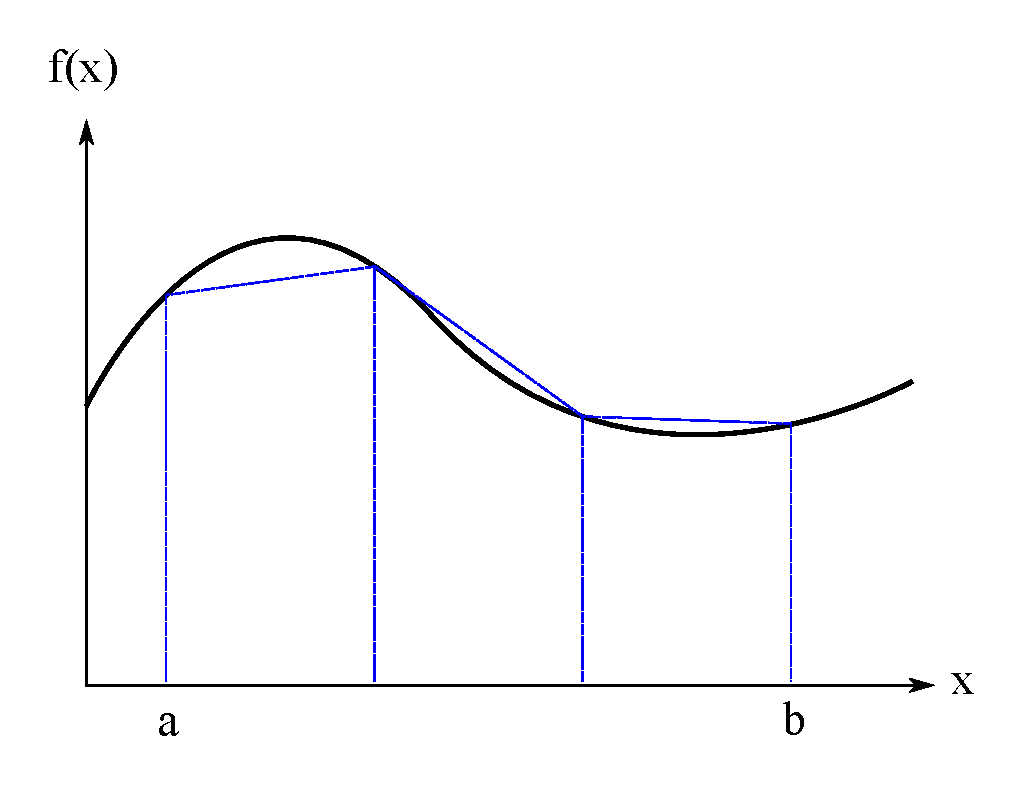
\includegraphics[width=8cm]{integral_diag.pdf}
\caption{Approximating $\int_{x=a}^{b} f(x)$ by summing the area of three trapezoids. }
\end{figure*}

Consider very simple numerical integration code, which tries to
compute $\int_{x=a}^{b} f(x)$ using $n$ steps:
% ./code/Trapezoid.hs
\begin{listing}
\begin{Verbatim}
module Main where

import System (getArgs)

main :: IO ()
main = do
  aStr:bStr:nStr:_ <- getArgs
  let [a,b] = map read [aStr,bStr]
      n = read nStr
      h = (b - a) / fromIntegral n
      integral = trapezoid f a b n h
  print integral 

-- Integrate 'f' on interval [a,b] using 'n' steps of size 'h'
trapezoid :: (Double -> Double) -> Double -> Double -> Int -> Double -> Double
trapezoid f a b n h =
  h * sum (endPoints:internals)
  where
  endPoints = (f a + f b) / 2
  internals = map f $ take (n - 1) $ iterate (+h) (a + h)

f :: Double -> Double
-- f x = 4 / (1 + x * x)
-- f = cos
f = const 1
\end{Verbatim}
\end{listing}

After splitting interval into arbitrary number of parts you could
integrate them separately and them sum the results. In fact, very
simple modification is required to make this code use all available
cores in single multi-cored machine:
\begin{Verbatim}
TODO: put threaded code here
\end{Verbatim}

But what if you want to do that on more that one box to utilise even
bigger number of cores? You would have, at the very least, tell the
processes on each node which part of the task they would work on, and
later on you would have to gather and combines results from them.

This could be done manually, but if you want to run the program
repeatedly, or if your interprocess communications are even slightly
more complex, you would need some means of communication between
processes. In pseudo-code, this would look like this:

\begin{Verbatim}
find number of available nodes
split interval between them
tell each node the interval it would work on
perform work (integration) on each node and send result to master node
collect results from nodes
sum them up
\end{Verbatim}

\ToDo: ideas for further sections: show how easy it would be to extend this to ``find number of nodes AND number of cores on them, split work according to power of node''


\section{Introducing haskell-mpi}

Good news! Pseudo-code from the previous section could be directly translated into haskell code:

%\begin{Verbatim}
%-- find number of available nodes
%nodes <- commSize commWorld
%-- split interval between them
%...
%-- tell each node the interval it would work on
%
%-- perform work (integration) on each node and send results to master node
%if node == master then gatherSend else gatherRecv ..
%-- collect results from nodes 
%-- sum them up
%total = sum results
%\end{Verbatim}

\begin{Verbatim}
module Main where

import Control.Parallel.MPI.Simple
import System (getArgs)

main :: IO ()
main = mpiWorld $ \numRanks rank -> do
  aStr:bStr:nStr:_ <- getArgs
  let [a,b] = map read [aStr,bStr]
      n = read nStr
      h = (b - a) / fromIntegral n
      localN = n `div` fromIntegral numRanks
      localA = a + fromIntegral rank * fromIntegral localN * h
      localB = localA + fromIntegral localN * h
      integral = trapezoid f localA localB localN h
  if rank == 0
     then print . sum =<< gatherRecv commWorld 0 integral
     else gatherSend commWorld 0 integral

trapezoid :: (Double -> Double) -> Double -> Double -> Int -> Double -> Double
trapezoid f a b n h =
  h * sum (endPoints:internals)
  where
  endPoints = (f a + f b) / 2
  internals = map f $ take (n - 1) $ iterate (+h) (a + h)

f :: Double -> Double
f x = 4 / (1 + x * x)
\end{Verbatim}
%% $ - for naive auctex mode that thiks that math mode somehow escapes
%% from Verbatim and rules over the rest of the text. AuCTeX, you are wrong!

\ToDo quickly introduce ``communicators'' and ``ranks'' here, refer readers to MPI docs and books for further reading (in footnote)

Messages could be sent from process to process or
dispatched to/from all process in a group, called in MPI terminology ``communicator''.

That was easy, isn't it? You can compile and run this code like this (assuming that you have OpenMPI installed): .... Please see Appendix A for installation and configuration hint, please see OpenMPI docs on how to tell OpenMPI where your nodes are. Even if you do development on a standalone box, it is easy to see that MPI would utilise several processes: ...

\section{Does this really speeds things up?}

You bet! We tried this code on ... and got those amazing results (table and graph):

\ToDo: measurement results here

You can see (describe something less obvious that could be derived from the graph).

\ToDo: we could also do this: We even took some less-trivial haskell
code (McPhd) and applied the same approach to parallelize it (href to
patch on git-hub) and here is what we've got: another table and graph.

\section{I'm hooked. What else could haskell-mpi do?}

You could use it to combine haskell and C code. Here is how: (separate sub-section on this?)
\subsection{Interacting with C}
\begin{Verbatim}
#include <mpi.h>
#include <stdio.h>
#include <stdlib.h>
#include <math.h>

double f(double);
double trapezoid(double, double, int, double);

int main(int argc, char **argv) {
   double a, b, h, local_a, local_b, integral, sum = 0;
   double *results = NULL;
   int n, local_n, rank, num_ranks;

   MPI_Init(&argc, &argv);
   MPI_Comm_size(MPI_COMM_WORLD, &num_ranks);
   MPI_Comm_rank(MPI_COMM_WORLD, &rank);

   a = atof(argv[1]);
   b = atof(argv[2]);
   n = atoi(argv[3]);

   h = (b - a) / n;
   local_n = n / num_ranks;
   local_a = a + rank * local_n * h;
   local_b = local_a + local_n * h;
   integral = trapezoid(local_a, local_b, local_n, h);

   if (rank == 0) {
      results = (double *) malloc(num_ranks * sizeof(double));
   }

   MPI_Gather(&integral, 1, MPI_DOUBLE, results, 1, MPI_DOUBLE, 0, MPI_COMM_WORLD);

   if (rank == 0) {
      for (int i = 0; i < num_ranks; i++) {
         sum += results[i];
      }
      printf("%lf\n", sum);
   }
   MPI_Finalize();
}

double trapezoid(double a, double b, int n, double h) {
   double result;
   double x = a;
   result = (f(a) + f(b)) / 2.0;
   for (int i = 1; i < n; i++) {
      x = x + h;
      result += f(x);
   }
   return result * h;
}

double f(double x) {
   return 4.0 / (1 + x * x);
}
\end{Verbatim}


Or you can you is to implement less trivial communication patterns (allreduce example or something more complex?)


\section{Conclusion, further reading, next steps, ...}

\ToDo mention somewhere bundled example and tests that could provide inspiration :)

\ToDo mention Well-Typed

\section{Appendix A: Installation and tested MPI implementations}
We tested the code on MPICH 1.2.x and 1.4.x, OpenMPI x.y.z. Amount of implementation-specific code is minimal and there is a good chance that all the other MPI implementations would be supported out of the box.

To install, try ``cabal install haskell-mpi''. If that fails to find MPI include/library files in system-wide directories, try ...
\ToDo provide installation cmdline

\bibliography{haskell-mpi}

\end{document}
